\documentclass{beamer}
% Required packages
\usepackage{amsmath}
\usepackage{physics}
\usepackage{graphicx}
\usepackage{siunitx}
\usepackage{xcolor}
% Define custom colors for DS9 theme
\definecolor{ds9blue}{RGB}{25,25,112}
\definecolor{ds9gold}{RGB}{218,165,32}
\definecolor{ds9grey}{RGB}{105,105,105}
\definecolor{ds9red}{RGB}{178,34,34}
% Set up the Madrid theme with custom colors
\usetheme{Madrid}
\usecolortheme{whale}
\setbeamercolor{palette primary}{bg=ds9blue,fg=white}
\setbeamercolor{palette secondary}{bg=ds9grey,fg=white}
\setbeamercolor{palette tertiary}{bg=ds9gold,fg=black}
\setbeamercolor{palette quaternary}{bg=ds9red,fg=white}
\setbeamercolor{structure}{fg=ds9blue}
\setbeamercolor{title}{fg=ds9gold}
\setbeamercolor{subtitle}{fg=ds9gold}
\setbeamercolor{frametitle}{bg=ds9blue,fg=white}
\setbeamercolor{block title}{bg=ds9blue,fg=white}
\setbeamercolor{block body}{bg=ds9grey!20,fg=black}

% Title page configuration
\title[EM Induction]{PHYS12 CH: 23.1-23.7}
\subtitle{Electromagnetic Induction and Its Applications}
\author[Mr. Gullo]{Mr. Gullo}
\date[April 2025]{April, 2025}

\begin{document}

% Title page
\begin{frame}
\titlepage
\end{frame}

% Table of contents
\begin{frame}
\frametitle{Outline}
\tableofcontents
\end{frame}

\section{Learning Objectives}

\begin{frame}
\frametitle{Learning Objectives}
By the end of this presentation, you will be able to:
\begin{itemize}
    \item Define magnetic flux and explain electromagnetic induction
    \item State and apply Faraday's Law and Lenz's Law
    \item Calculate motional emf in a conductor moving through a magnetic field
    \item Explain the concepts of eddy currents and magnetic damping
    \item Describe the operation of electric generators
    \item Understand the concept of back emf in motors
    \item Analyze transformer operation and calculate voltage/current relationships
\end{itemize}
\end{frame}

\section{Magnetic Flux and Induction}

\begin{frame}
\frametitle{Magnetic Flux}
\begin{block}{Definition}
Magnetic flux ($\Phi$) is a measure of the total magnetic field passing through a given area.
\end{block}

\begin{columns}
\column{0.5\textwidth}
\begin{align}
\Phi &= BA\cos\theta \\
\text{where:} \\
B &= \text{magnetic field strength} \\
A &= \text{area} \\
\theta &= \text{angle with perpendicular}
\end{align}

\column{0.5\textwidth}
\begin{itemize}
\item Units: Tesla·meter² (T·m²)
\item Maximum when $\theta = 0°$ (field perpendicular to area)
\item Zero when $\theta = 90°$ (field parallel to area)
\end{itemize}
\end{columns}


\end{frame}

\begin{frame}
\begin{figure}
    \centering
    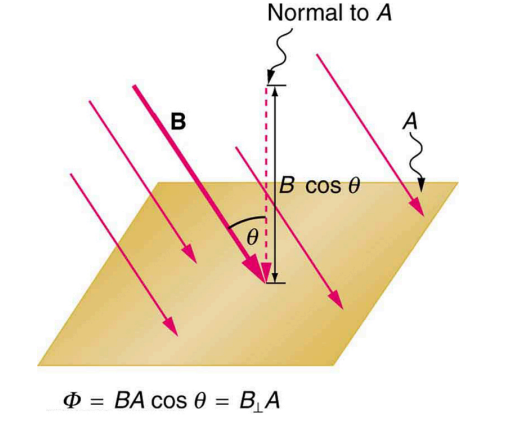
\includegraphics[width=0.8\linewidth]{mangle.png}
\end{figure}

\end{frame}

\begin{frame}
\frametitle{Electromagnetic Induction}
\begin{block}{Fundamental Principle}
Any change in magnetic flux induces an electromotive force (emf).
\end{block}

\begin{itemize}
\item Discovered independently by Michael Faraday and Joseph Henry
\item The induced emf can drive current through a circuit
\item The induced current creates its own magnetic field
\item Basis for generators, transformers, and many electrical devices
\end{itemize}

\begin{alertblock}{Key Insight}
It's the \textbf{change} in magnetic flux that induces emf, not the flux itself.
\end{alertblock}

\alert{[\href{https://phet.colorado.edu/en/simulations/faraday}{PHET showing a magnet moving through a coil and the resulting induced current}]}
\end{frame}

\section{Faraday's Law and Lenz's Law}

\begin{frame}
\frametitle{Faraday's Law of Induction}
\begin{block}{Mathematical Form}
\begin{align}
\text{emf} = -N\frac{\Delta\Phi}{\Delta t}
\end{align}
\end{block}

\begin{columns}
\column{0.6\textwidth}
\begin{itemize}
\item $N$ = number of turns in a coil
\item $\Delta\Phi$ = change in magnetic flux
\item $\Delta t$ = time interval for the change
\item The negative sign is due to Lenz's Law
\end{itemize}

\column{0.4\textwidth}
\begin{itemize}
\item Ways to change flux:
\begin{itemize}
    \item Change $B$ (field strength)
    \item Change $A$ (area)
    \item Change $\theta$ (orientation)
\end{itemize}
\end{itemize}
\end{columns}
\end{frame}

\begin{frame}
\begin{figure}
    \centering
    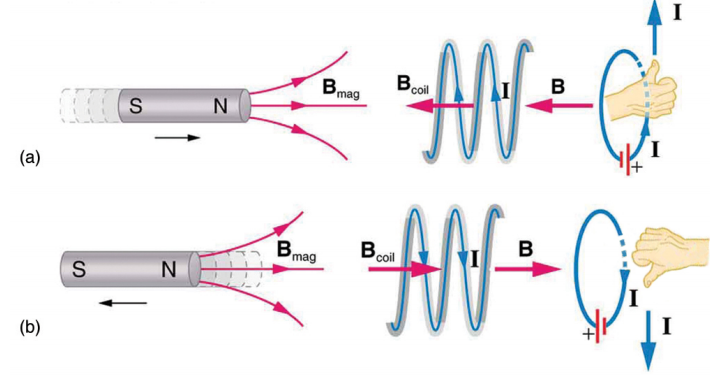
\includegraphics[width=0.75\linewidth]{chflux.png}
\end{figure}
\end{frame}

\begin{frame}
\frametitle{Lenz's Law}
\begin{block}{The Minus Sign in Faraday's Law}
The induced emf creates a current that produces a magnetic field opposing the change in flux that induced it.
\end{block}

\begin{itemize}
\item Conservation of energy principle
\item If flux is increasing, induced field opposes the increase
\item If flux is decreasing, induced field opposes the decrease
\item Works against the cause of the flux change
\end{itemize}

\begin{alertblock}{Important Note}
Lenz's Law explains why work must be done against the induced magnetic force to maintain flux changes.
\end{alertblock}


\end{frame}

\section{Types of Induced EMF}

\begin{frame}
\frametitle{Motional EMF}
\begin{block}{Definition}
EMF induced by motion of a conductor through a magnetic field.
\end{block}

\begin{columns}
\column{0.5\textwidth}
For a straight conductor:
\begin{align}
\text{emf} = B\ell v
\end{align}

\begin{itemize}
\item $B$ = magnetic field strength
\item $\ell$ = length of conductor
\item $v$ = velocity of conductor
\end{itemize}

\column{0.5\textwidth}
\begin{itemize}
\item Applies when $B$, $\ell$, and $v$ are mutually perpendicular
\item Causes charge separation in the conductor
\item Creates potential difference across the conductor
\end{itemize}
\end{columns}
\end{frame}

\begin{frame}
\begin{figure}
    \centering
    \includegraphics[width=0.75\linewidth]{emfmage.png}
\end{figure}
\end{frame}

\begin{frame}
\frametitle{Eddy Currents}
\begin{block}{Definition}
Current loops induced in moving conductors or changing magnetic fields.
\end{block}

\begin{columns}
\column{0.5\textwidth}
\begin{itemize}
\item Occur in solid conductors moving through magnetic fields
\item Flow in closed loops within the conductor
\item Can cause significant heating (I²R losses)
\item Used in induction heating and cooking
\end{itemize}

\column{0.5\textwidth}
\begin{itemize}
\item \textbf{Magnetic Damping}:
\begin{itemize}
    \item Drag force from eddy currents
    \item Opposes the motion that created it
    \item Used in braking systems
    \item Can be reduced by slotting conductors
\end{itemize}
\end{itemize}
\end{columns}
\end{frame}

\begin{frame}
\begin{figure}
    \centering
    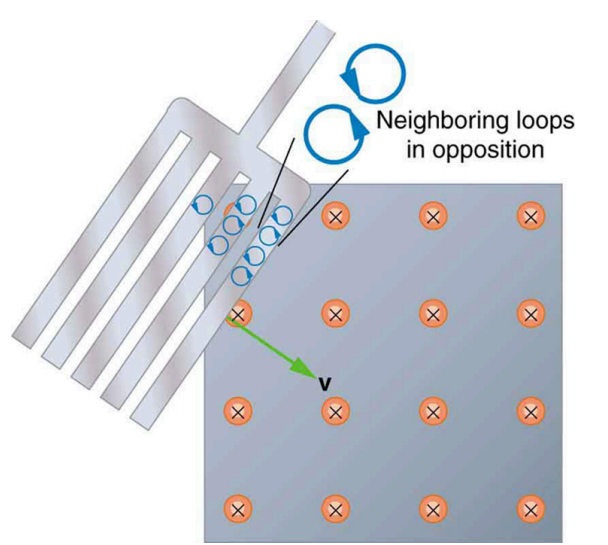
\includegraphics[width=0.5\linewidth]{eddy.png}
\end{figure}

\end{frame}

\section{Devices Based on Induction}

\begin{frame}
\frametitle{Electric Generators}
\begin{block}{Working Principle}
A coil rotating in a magnetic field induces a time-varying emf.
\end{block}

\begin{columns}
\column{0.5\textwidth}
\begin{align}
\text{emf} &= NAB\omega\sin(\omega t) \\
\text{where:} \\
N &= \text{number of turns} \\
A &= \text{area of coil} \\
B &= \text{magnetic field strength} \\
\omega &= \text{angular velocity}
\end{align}

\column{0.5\textwidth}
\begin{itemize}
\item Peak emf: $\text{emf}_0 = NAB\omega$
\item Produces sinusoidal AC voltage
\item Converts mechanical energy to electrical energy
\item Basis for power generation worldwide
\end{itemize}
\end{columns}

\end{frame}

\begin{frame}
\begin{figure}
    \centering
    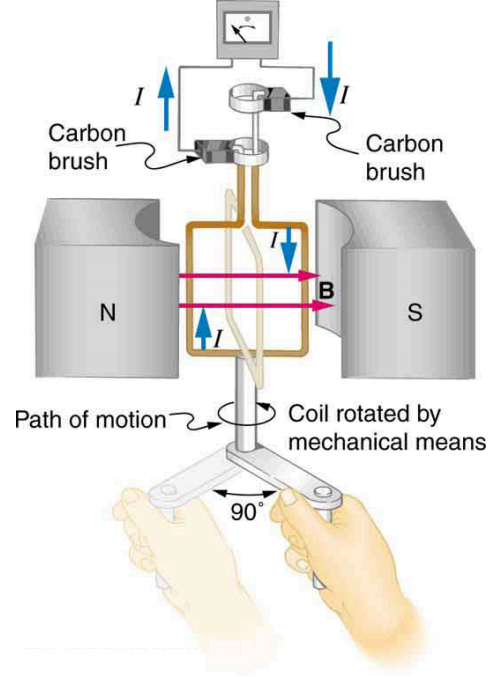
\includegraphics[width=0.6\linewidth]{genyr.png}
\end{figure}
\end{frame}

\begin{frame}
\frametitle{Back EMF in Motors}
\begin{block}{Definition}
Induced emf in a motor that opposes the applied voltage.
\end{block}

\begin{itemize}
\item Motors are generators in reverse: convert electrical to mechanical energy
\item When a motor rotates, it also acts as a generator
\item This self-generated emf opposes the applied voltage
\item Magnitude increases with motor speed
\item Limits current in a running motor
\item Back emf = 0 when motor is first starting (why starting current is high)
\end{itemize}

\begin{alertblock}{Safety Note}
The high starting current is why motors need special starters or current limiters.
\end{alertblock}

\end{frame}

\begin{frame}
\frametitle{Transformers}
\begin{block}{Basic Purpose}
Transform AC voltage from one value to another using electromagnetic induction.
\end{block}

\begin{columns}
\column{0.5\textwidth}
\textbf{Voltage Relationship:}
\begin{align}
\frac{V_s}{V_p} = \frac{N_s}{N_p}
\end{align}

\textbf{Current Relationship:}
\begin{align}
\frac{I_s}{I_p} = \frac{N_p}{N_s}
\end{align}

\column{0.5\textwidth}
\begin{itemize}
\item Primary coil: Connected to AC source
\item Secondary coil: Delivers transformed voltage
\item $N_p, N_s$: Number of turns in primary and secondary
\item $V_p, V_s$: Primary and secondary voltages
\item $I_p, I_s$: Primary and secondary currents
\end{itemize}
\end{columns}

\begin{itemize}
\item \textbf{Step-up transformer:} $N_s > N_p$ (increases voltage, decreases current)
\item \textbf{Step-down transformer:} $N_s < N_p$ (decreases voltage, increases current)
\end{itemize}

\alert{[Cross-sectional diagram of a transformer showing primary and secondary coils]}
\end{frame}

\section{Practical Applications}

\begin{frame}
\frametitle{Example Problem: "I do"}
\begin{block}{Motional EMF Problem}
A metal rod of length 1.0 m moves at 2.0 m/s perpendicular to a magnetic field of 0.50 T. Calculate the induced emf.
\end{block}

\begin{itemize}
\item \textbf{Given:}
\begin{itemize}
    \item Length of rod: $\ell = 1.0 \text{ m}$
    \item Speed of rod: $v = 2.0 \text{ m/s}$
    \item Magnetic field: $B = 0.50 \text{ T}$
\end{itemize}
\item \textbf{Find:} The induced emf
\end{itemize}

\pause

\begin{align}
\text{emf} &= B\ell v \\
&= (0.50 \text{ T})(1.0 \text{ m})(2.0 \text{ m/s}) \\
&= 1.0 \text{ V}
\end{align}


\end{frame}

\begin{frame}
\frametitle{Example Problem: "We do"}
\begin{block}{Generator Problem}
A generator has 100 turns of wire in a coil with area 0.05 m² and rotates in a magnetic field of 0.75 T at 60 Hz. Calculate the peak emf.
\end{block}

\begin{itemize}
\item \textbf{Given:}
\begin{itemize}
    \item Number of turns: $N = 100$
    \item Area of coil: $A = 0.05 \text{ m}^2$
    \item Magnetic field: $B = 0.75 \text{ T}$
    \item Frequency: $f = 60 \text{ Hz}$
\end{itemize}
\item \textbf{Find:} The peak emf ($\text{emf}_0$)
\end{itemize}

Let's work through this together:
\begin{align}
\omega &= 2\pi f = 2\pi(60 \text{ Hz}) = 377 \text{ rad/s} \\
\text{emf}_0 &= NAB\omega \\
&= 100 \times 0.05 \text{ m}^2 \times 0.75 \text{ T} \times 377 \text{ rad/s} \\
&= ?
\end{align}
\end{frame}

\begin{frame}
\frametitle{Example Problem: "You do"}
\begin{block}{Transformer Problem}
A transformer has 400 primary turns and 100 secondary turns. If the primary voltage is 120 V, what is the secondary voltage?
\end{block}

\begin{itemize}
\item \textbf{Given:}
\begin{itemize}
    \item Primary turns: $N_p = 400$
    \item Secondary turns: $N_s = 100$
    \item Primary voltage: $V_p = 120 \text{ V}$
\end{itemize}
\item \textbf{Find:} Secondary voltage ($V_s$)
\end{itemize}

\begin{alertblock}{Hint}
Use the voltage relationship for transformers: $\frac{V_s}{V_p} = \frac{N_s}{N_p}$
\end{alertblock}

Try to solve this problem on your own!
\end{frame}

\section{Summary}

\begin{frame}
\frametitle{Key Equations}
\begin{table}
\begin{tabular}{ll}
\hline
\textbf{Concept} & \textbf{Equation} \\
\hline
Magnetic Flux & $\Phi = BA\cos\theta$ \\
Faraday's Law & $\text{emf} = -N\frac{\Delta\Phi}{\Delta t}$ \\
Motional EMF & $\text{emf} = B\ell v$ \\
Generator EMF & $\text{emf} = NAB\omega\sin(\omega t)$ \\
Peak Generator EMF & $\text{emf}_0 = NAB\omega$ \\
Transformer Voltage & $\frac{V_s}{V_p} = \frac{N_s}{N_p}$ \\
Transformer Current & $\frac{I_s}{I_p} = \frac{N_p}{N_s}$ \\
\hline
\end{tabular}
\end{table}
\end{frame}

\begin{frame}
\frametitle{Summary of Key Concepts}
\begin{itemize}
\item \textbf{Electromagnetic Induction:} Process by which changing magnetic flux induces an emf
\item \textbf{Faraday's Law:} Quantifies the relationship between changing flux and induced emf
\item \textbf{Lenz's Law:} Determines the direction of induced current to oppose the change
\item \textbf{Motional EMF:} Produced when a conductor moves through a magnetic field
\item \textbf{Eddy Currents:} Closed loops of current induced in solid conductors
\item \textbf{Generators:} Convert mechanical energy to electrical energy using induction
\item \textbf{Back EMF:} Self-induced voltage in motors that opposes applied voltage
\item \textbf{Transformers:} Convert AC voltage levels using mutual induction
\end{itemize}
\end{frame}

\begin{frame}
\frametitle{Real-World Applications}
\begin{columns}
\column{0.5\textwidth}
\begin{block}{Power Generation \& Distribution}
\begin{itemize}
\item Electric generators in power plants
\item Step-up transformers at power plants
\item Step-down transformers near consumers
\end{itemize}
\end{block}

\begin{block}{Transportation}
\begin{itemize}
\item Electric motors in vehicles
\item Magnetic braking systems
\item Induction sensors
\end{itemize}
\end{block}

\column{0.5\textwidth}
\begin{block}{Consumer Electronics}
\begin{itemize}
\item Induction cooktops
\item Wireless charging systems
\item Microphones and speakers
\end{itemize}
\end{block}

\begin{block}{Medical Technology}
\begin{itemize}
\item MRI machines
\item Electromagnetic flow meters
\item Transcranial magnetic stimulation
\end{itemize}
\end{block}
\end{columns}
\end{frame}

\begin{frame}
\frametitle{Questions?}
\begin{center}
\Large Thank you for your attention!

\vspace{1cm}

Any questions?
\end{center}
\end{frame}

\end{document}